\setcounter{figure}{0}
\setcounter{table}{0}
\setcounter{equation}{0}
\section{误差理论与数据处理系统实验分析}
根据前面界面的设计,已经编写好所有界面。整个系统包括测量数据基本处理、误差的合成、测量不确定度、最小二乘法处理、回归分析五个部分,算法的设计都是根据前面第一部分的误差理论与数据处理的理论知识来完成的。
\begin{figure}[H]
	\centering
	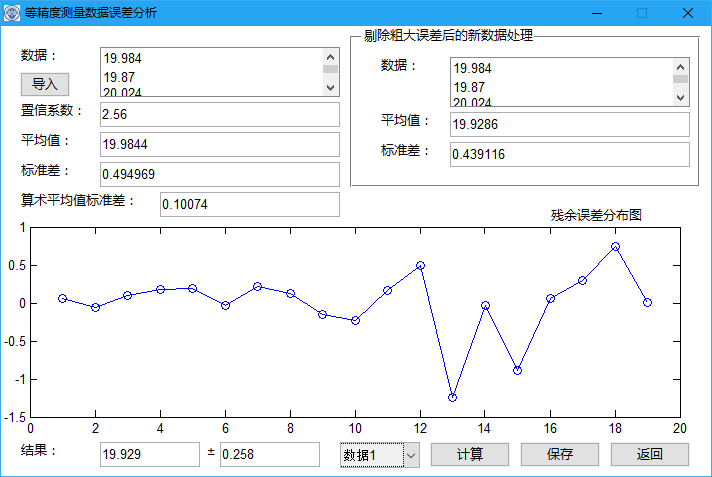
\includegraphics[scale=0.5]{subsubpage1_1}
	\caption{\textbf{等精度测量数据误差分析界面}}
\end{figure}
\subsection{等精度测量数据误差分析}
已编写好系统中等精度测量数据误差分析的界面如图3-1。该系统可以导入、处理、显示和保存数据,导入是使用load函数和xlsread函数来导入txt数据文件和Excel数据文件,保存则使用xlswrite函数来保存在Excel表格文件中,处理数据后的结果如图3-1。计算的功能是编写在计算按钮的回调函数中,子函数代码如下:
\begin{lstlisting}
 function run1(cbo,handles)							% 计算按钮的回调函数
 handles = guidata(cbo);							% 获取存储的 GUI 数据
 s1 = str2num(get(handles.data,'String'));			% 获取数据文本框的数据并转换为数字
 s2 = str2num(get(handles.coefficient,'String'));	% 获取置信系数并转换为数字
 if isempty(s1)||isempty(s2)						% 计算前判断数据是否为空
	 warndlg('缺少输入参数!');
	 return;
 end
 [data1,v1,a,a1,s,s1,s1_x,x] = data_process1(s1,s2);% 调用数据处理m函数文件
 axes(handles.axes);								% 指定坐标轴
 plot(v1,'-o');										% 绘制残余误差分布图
 set(handles.data_,'String',data1);					% 将计算结果显示到文本框
 set(handles.average,'String',a);
 set(handles.average_,'String',a1);
 set(handles.standard,'String',s);
 set(handles.standard_,'String',s1);
 set(handles.average_standard,'String',s1_x);
 set(handles.result_1,'String',x(1));
 set(handles.result_2,'String',x(2));\end{lstlisting}
 
上面用到的data\_process1等数度测量数据误差分析函数,等精度误差分析的过程如图1-1,代码如下:
\begin{lstlisting}
 function [data1,v1,a,a1,s,s1,s1_x,x] = data_process1(data,t_a)
 a = mean(data);									% 原数据平均值
 s = std(data);										% 原数据标准差
 data1 = BlodBig(data);								% 去除粗大误差后的数据
 a1 = mean(data1);									% 去除粗大误差后数据平均值
 s1 = std(data1);									% 去除粗大误差后数据标准差
 n1 = length(data1);								% 去除粗大误差后数据长度
 v1 = 1:n1;
 for i=1:n1
 v1(i) = data1(i)-a1;								% 残余误差
 end
 s1_x = s1/sqrt(n1);								% 算术平均值标准差
 sigama = t_a*s1_x;									% 算术平均值极限误差
 x = roundn([a1 sigama],-3);						% 四舍五入保留三位小数结果\end{lstlisting}

上面使用的狄克逊准则剔除粗大误差算法BlodBig.m函数文件代码如下:
\begin{lstlisting}
 function data1 = BlodBig(data)
 % a=0.05 的临界值
 r0 = [0 0 0.941 0.765 0.642 0.560 0.507 0.554 0.512 0.447 0.576 0.546 0.521 0.548 0.525 0.507 0.490 0.475 0.462 0.450 0.440 0.430 0.421 0.413 0.406 0.399 0.393 0.387 0.381 0.378];  
 n = length(data);									% 数据的长度
 data_ = sort(data);								% 排序后的数据
 if n<3												% 数据太少不进行剔除
 msgbox('数据太少','提示','warn');
 data1 = data;
 return
 elseif n>=3 && n<=7								% 狄克逊准则判别粗大误差
 r = (data_(n)-data_(n-1))/(data_(n)-data_(1));
 r_ = (data_(1)-data_(2))/(data_(1)-data_(n));
 elseif n>=8 && n<=10
 r = (data_(n)-data_(n-1))/(data_(n)-data_(2));
 r_ = (data_(1)-data_(2))/(data_(1)-data_(n-1));
 elseif n>=11 && n<=13
 r = (data_(n)-data_(n-2))/(data_(n)-data_(2));
 r_ = (data_(1)-data_(3))/(data_(1)-data_(n-1));
 else
 r = (data_(n)-data_(n-2))/(data_(n)-data_(3));
 r_ = (data_(1)-data_(3))/(data_(1)-data_(n-2));
 end
 if r>=r0(n)
 data(data==data_(n)) = [];							% 剔除粗大误差
 elseif r_>=r0(n)
 data(data==data_(1)) = [];							% 剔除粗大误差
 end
 data1 = data;										% 返回剔除粗大误差的数据\end{lstlisting}
\subsection{回归系统实验分析}
不等精度测量数据误差分析、误差的合成、测量不确定度和最小二乘法处理的算法详情见附录D,回归分析的界面已经设计好如图3-2。
\begin{figure}[H]
	\centering
	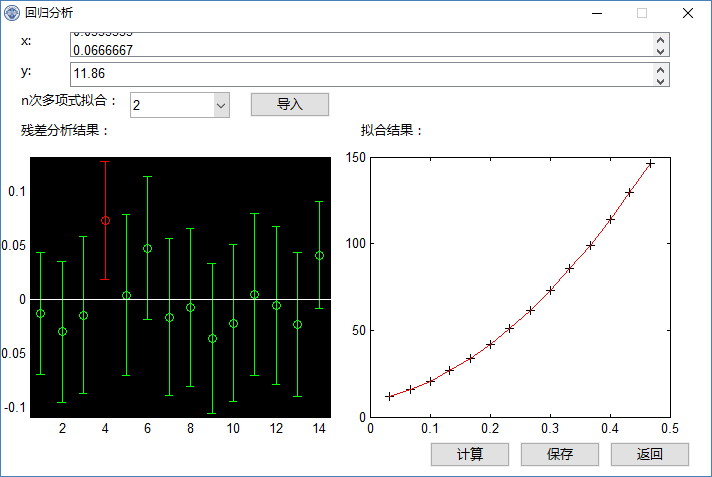
\includegraphics[scale=0.5]{subsubpage5}
	\caption{\textbf{回归分析界面}}
\end{figure}

界面中,导入按钮可以实现导入Excel数据的功能,计算按钮的回调函数代码如下:
\begin{lstlisting}
 function run1(cbo,handles)							% 回调函数
 handles = guidata(cbo);							% 获取界面数据
 x = str2num(get(handles.x,'String'));
 y = str2num(get(handles.y,'String'));
 l = size(x);
 if l(1)>1
 x = x';
 y = y';
 end
 n = get(handles.list,'Value');
 if isempty(x)||isempty(y)							% 判断输入数据是否为空
	 warndlg('缺少输入参数!');
	 return;
 end
 I = ones(length(x),1);
 for i=1:n
 b = x.^i;
 I = [I b'];
 end
 [b,bint,r,rint,stats]=regress(y',I);
 axes(handles.v_axes);
 rcoplot(r,rint);
 title('');
 xlabel('');
 ylabel('');
 Y = polyval(b(end:-1:1),x);						% 绘制回归曲线
 axes(handles.r_axes);
 plot(x,y,'k+',x,Y,'r');\end{lstlisting}

该界面主要利用regress函数能实现数据的多次函数回归拟合保存按钮可以保存绘制好的残差分析结果图和拟合结果图,进行回归处理后得到的图像如图3-2。